\documentclass[a4paper]{book}
\usepackage{a4wide}
\usepackage{makeidx}
\usepackage{fancyhdr}
\usepackage{graphicx}
\usepackage{multicol}
\usepackage{float}
\usepackage{textcomp}
\usepackage{alltt}
\usepackage{times}
\usepackage{ifpdf}
\ifpdf
\usepackage[pdftex,
            pagebackref=true,
            colorlinks=true,
            linkcolor=blue,
            unicode
           ]{hyperref}
\else
\usepackage[ps2pdf,
            pagebackref=true,
            colorlinks=true,
            linkcolor=blue,
            unicode
           ]{hyperref}
\usepackage{pspicture}
\fi
\usepackage[utf8]{inputenc}
\usepackage{doxygen}
\makeindex
\setcounter{tocdepth}{3}
\renewcommand{\footrulewidth}{0.4pt}
\begin{document}
\begin{titlepage}
\vspace*{7cm}
\begin{center}
{\Large Reference Manual}\\
\vspace*{1cm}
{\large Generated by Doxygen 1.5.6}\\
\vspace*{0.5cm}
{\small Sat Oct 18 10:41:36 2008}\\
\end{center}
\end{titlepage}
\clearemptydoublepage
\pagenumbering{roman}
\tableofcontents
\clearemptydoublepage
\pagenumbering{arabic}
\chapter{Class Index}
\section{Class Hierarchy}
This inheritance list is sorted roughly, but not completely, alphabetically:\begin{CompactList}
\item \contentsline{section}{PObject}{\pageref{classPObject}}{}
\begin{CompactList}
\item \contentsline{section}{POSphere}{\pageref{classPOSphere}}{}
\end{CompactList}
\end{CompactList}

\chapter{Class Index}
\section{Class List}
Here are the classes, structs, unions and interfaces with brief descriptions:\begin{CompactList}
\item\contentsline{section}{\hyperlink{classPObject}{PObject} (The base class for all Physics Objects )}{\pageref{classPObject}}{}
\item\contentsline{section}{\hyperlink{classPOSphere}{POSphere} (Class for sphere Physics Objects )}{\pageref{classPOSphere}}{}
\end{CompactList}

\chapter{Class Documentation}
\hypertarget{classPObject}{
\section{PObject Class Reference}
\label{classPObject}\index{PObject@{PObject}}
}
The base class for all Physics Objects.  


{\tt \#include $<$pobject.h$>$}

Inheritance diagram for PObject::\begin{figure}[H]
\begin{center}
\leavevmode
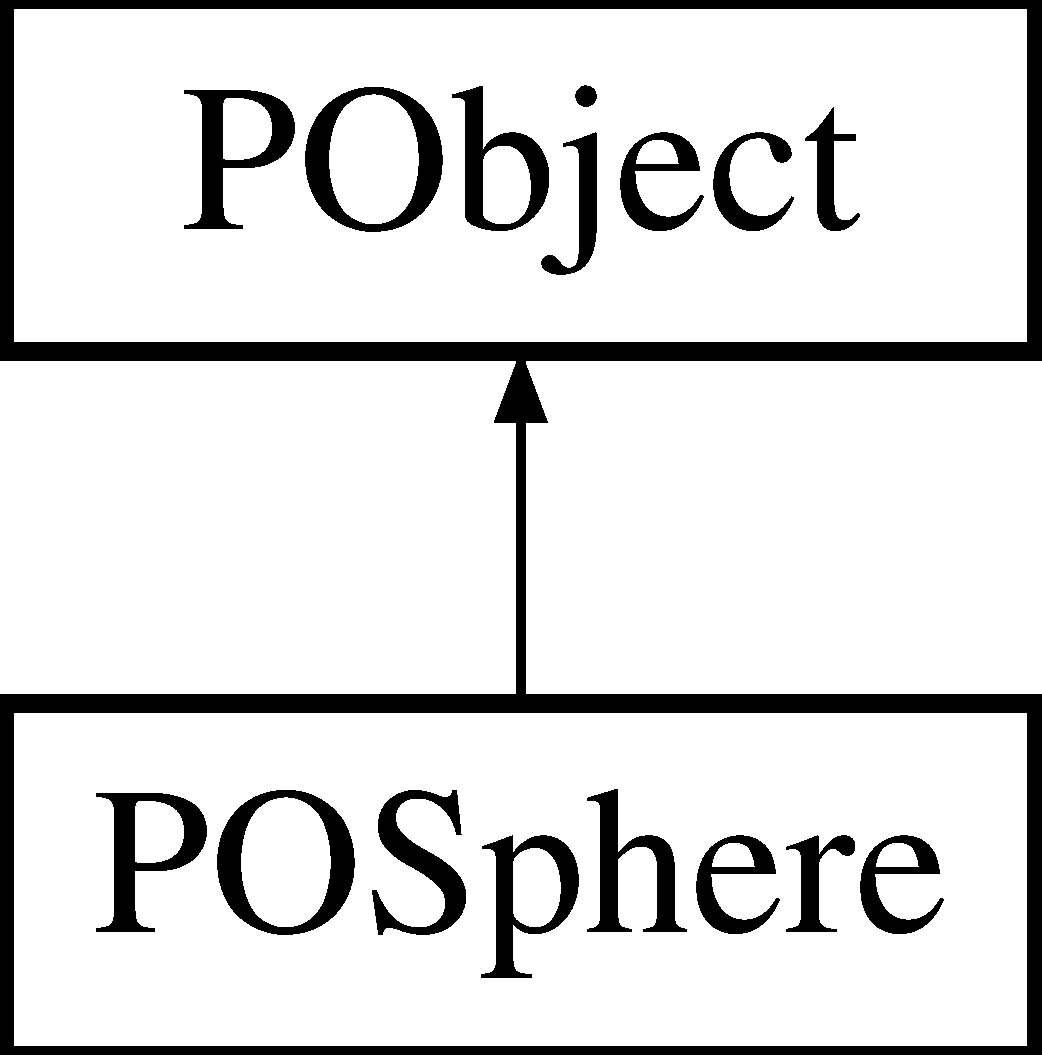
\includegraphics[height=2cm]{classPObject}
\end{center}
\end{figure}
\subsection*{Public Member Functions}
\begin{CompactItemize}
\item 
\hypertarget{classPObject_21d0fc7628b6f59bfa24caccff0de01a}{
\hyperlink{classPObject_21d0fc7628b6f59bfa24caccff0de01a}{$\sim$PObject} ()}
\label{classPObject_21d0fc7628b6f59bfa24caccff0de01a}

\begin{CompactList}\small\item\em default base constructer \item\end{CompactList}\item 
virtual void \hyperlink{classPObject_587e0263ce46133bf886729f890f9f2b}{update} ()=0
\begin{CompactList}\small\item\em default base destructer \item\end{CompactList}\item 
virtual Scalar \hyperlink{classPObject_e1828c1830e8e9924ca4c560cbe2f933}{detectCollision} (\hyperlink{classPObject}{PObject} $\ast$object)=0
\begin{CompactList}\small\item\em pure virtual detect collision \item\end{CompactList}\item 
virtual varList \hyperlink{classPObject_4def469478987ead107c777d31790092}{getStats} ()=0
\begin{CompactList}\small\item\em pure virtual get Statistics for the object \item\end{CompactList}\item 
\hypertarget{classPObject_b838f7867acec8e4199947aaf51f9763}{
virtual void \hyperlink{classPObject_b838f7867acec8e4199947aaf51f9763}{setStats} (varList \_\-stats)=0}
\label{classPObject_b838f7867acec8e4199947aaf51f9763}

\begin{CompactList}\small\item\em pure virtual set stats \item\end{CompactList}\item 
\hypertarget{classPObject_d691c89b796676824080d00633e7f6f4}{
Vector$<$ Scalar $>$ \textbf{getPoM} ()}
\label{classPObject_d691c89b796676824080d00633e7f6f4}

\item 
\hypertarget{classPObject_bdca63793b7e6e59b568d157f7c8142f}{
void \hyperlink{classPObject_bdca63793b7e6e59b568d157f7c8142f}{setPoM} (Vector$<$ Scalar $>$ \_\-PoM)}
\label{classPObject_bdca63793b7e6e59b568d157f7c8142f}

\begin{CompactList}\small\item\em get Point of Mass \item\end{CompactList}\item 
\hypertarget{classPObject_9aa1ffb42bf4077cf69d2c4c8f11e839}{
Scalar \hyperlink{classPObject_9aa1ffb42bf4077cf69d2c4c8f11e839}{getMass} ()}
\label{classPObject_9aa1ffb42bf4077cf69d2c4c8f11e839}

\begin{CompactList}\small\item\em set Point of Mass \item\end{CompactList}\item 
\hypertarget{classPObject_f5f14a756807d0971641ebcbfc3e09f6}{
void \hyperlink{classPObject_f5f14a756807d0971641ebcbfc3e09f6}{setMass} (Scalar \_\-m)}
\label{classPObject_f5f14a756807d0971641ebcbfc3e09f6}

\begin{CompactList}\small\item\em get Mass \item\end{CompactList}\item 
\hypertarget{classPObject_b129b61f46fa06b9c17b9427e9aa2c48}{
Vector$<$ Scalar $>$ \hyperlink{classPObject_b129b61f46fa06b9c17b9427e9aa2c48}{getVelocity} ()}
\label{classPObject_b129b61f46fa06b9c17b9427e9aa2c48}

\begin{CompactList}\small\item\em set Mass \item\end{CompactList}\item 
\hypertarget{classPObject_d74f0ee87f3c5ae65f6403d63d6f1598}{
void \hyperlink{classPObject_d74f0ee87f3c5ae65f6403d63d6f1598}{setVelocity} (Vector$<$ Scalar $>$ \_\-vel)}
\label{classPObject_d74f0ee87f3c5ae65f6403d63d6f1598}

\begin{CompactList}\small\item\em get Velocity \item\end{CompactList}\item 
\hypertarget{classPObject_c336d4c39dade7245b02ff4c419626fb}{
Scalar \hyperlink{classPObject_c336d4c39dade7245b02ff4c419626fb}{getAccel} ()}
\label{classPObject_c336d4c39dade7245b02ff4c419626fb}

\begin{CompactList}\small\item\em set Velocity \item\end{CompactList}\item 
\hypertarget{classPObject_f2741df535880f8487386e67a547c276}{
void \hyperlink{classPObject_f2741df535880f8487386e67a547c276}{setAccel} (Scalar \_\-accel)}
\label{classPObject_f2741df535880f8487386e67a547c276}

\begin{CompactList}\small\item\em get Acceloration \item\end{CompactList}\item 
\hypertarget{classPObject_b89f4243fb28114546dee8a2247951ad}{
Scalar \hyperlink{classPObject_b89f4243fb28114546dee8a2247951ad}{getMMoI} ()}
\label{classPObject_b89f4243fb28114546dee8a2247951ad}

\begin{CompactList}\small\item\em set Acceloration \item\end{CompactList}\item 
\hypertarget{classPObject_5da6ef823f5791ede8b2a8cdc1fc18fb}{
void \hyperlink{classPObject_5da6ef823f5791ede8b2a8cdc1fc18fb}{setMMoI} (Scalar \_\-mmoi)}
\label{classPObject_5da6ef823f5791ede8b2a8cdc1fc18fb}

\begin{CompactList}\small\item\em get Mass Moment of Inertia \item\end{CompactList}\end{CompactItemize}
\subsection*{Protected Attributes}
\begin{CompactItemize}
\item 
Vector$<$ Scalar $>$ \hyperlink{classPObject_c605ad1786c7e60dc03faa7340e6b204}{PoM}
\begin{CompactList}\small\item\em set Mass Moment of Inertia \item\end{CompactList}\item 
\hypertarget{classPObject_b431b6b513a0f702fbcacda37cf0f3d3}{
Scalar \hyperlink{classPObject_b431b6b513a0f702fbcacda37cf0f3d3}{mass}}
\label{classPObject_b431b6b513a0f702fbcacda37cf0f3d3}

\begin{CompactList}\small\item\em Mass. \item\end{CompactList}\item 
\hypertarget{classPObject_d4676288b887b76c23405b2d0d88b652}{
Vector$<$ Scalar $>$ \hyperlink{classPObject_d4676288b887b76c23405b2d0d88b652}{velocity}}
\label{classPObject_d4676288b887b76c23405b2d0d88b652}

\begin{CompactList}\small\item\em Velocity. \item\end{CompactList}\item 
\hypertarget{classPObject_3b27cd99ff41d8f17770b125f43ebc9c}{
Scalar \hyperlink{classPObject_3b27cd99ff41d8f17770b125f43ebc9c}{acceloration}}
\label{classPObject_3b27cd99ff41d8f17770b125f43ebc9c}

\begin{CompactList}\small\item\em Acceloration. \item\end{CompactList}\item 
\hypertarget{classPObject_39549ad19aaa12033ae1c2bba1098f34}{
Scalar \hyperlink{classPObject_39549ad19aaa12033ae1c2bba1098f34}{MassMomentOfInertia}}
\label{classPObject_39549ad19aaa12033ae1c2bba1098f34}

\begin{CompactList}\small\item\em Mass Moment of Inertia. \item\end{CompactList}\end{CompactItemize}


\subsection{Detailed Description}
The base class for all Physics Objects. 

This is the math base for the mathematic simplistic representation of all physics based objects 

\subsection{Member Function Documentation}
\hypertarget{classPObject_587e0263ce46133bf886729f890f9f2b}{
\index{PObject@{PObject}!update@{update}}
\index{update@{update}!PObject@{PObject}}
\subsubsection[update]{\setlength{\rightskip}{0pt plus 5cm}virtual void PObject::update ()\hspace{0.3cm}{\tt  \mbox{[}pure virtual\mbox{]}}}}
\label{classPObject_587e0263ce46133bf886729f890f9f2b}


default base destructer 

pure virtual update 

Implemented in \hyperlink{classPOSphere_17904f3eeceb2ba07931d6d359bbeebe}{POSphere}.\hypertarget{classPObject_e1828c1830e8e9924ca4c560cbe2f933}{
\index{PObject@{PObject}!detectCollision@{detectCollision}}
\index{detectCollision@{detectCollision}!PObject@{PObject}}
\subsubsection[detectCollision]{\setlength{\rightskip}{0pt plus 5cm}virtual Scalar PObject::detectCollision ({\bf PObject} $\ast$ {\em object})\hspace{0.3cm}{\tt  \mbox{[}pure virtual\mbox{]}}}}
\label{classPObject_e1828c1830e8e9924ca4c560cbe2f933}


pure virtual detect collision 

This is the function that we will use to figure out the distance from another object and thus if we collided with it \begin{Desc}
\item[Returns:]Scalar value that is $>$0 if there is no collision =0 if they are just touching and $<$0 if they have hit to intersection(hit with force) \end{Desc}
\begin{Desc}
\item[Parameters:]
\begin{description}
\item[{\em brings}]in a pointer to a physics object to test for distance/collision \end{description}
\end{Desc}


Implemented in \hyperlink{classPOSphere_798625bc33390f84032dd30b5abaa112}{POSphere}.\hypertarget{classPObject_4def469478987ead107c777d31790092}{
\index{PObject@{PObject}!getStats@{getStats}}
\index{getStats@{getStats}!PObject@{PObject}}
\subsubsection[getStats]{\setlength{\rightskip}{0pt plus 5cm}virtual varList PObject::getStats ()\hspace{0.3cm}{\tt  \mbox{[}pure virtual\mbox{]}}}}
\label{classPObject_4def469478987ead107c777d31790092}


pure virtual get Statistics for the object 

This is the function that we will use to get the object's data for the objects \begin{Desc}
\item[Returns:]returns a list of stats. The first is the type ID. \end{Desc}
\begin{Desc}
\item[Parameters:]
\begin{description}
\item[{\em none}]\end{description}
\end{Desc}


Implemented in \hyperlink{classPOSphere_cab4d5434c63870cd383d38eb985a4fd}{POSphere}.

\subsection{Member Data Documentation}
\hypertarget{classPObject_c605ad1786c7e60dc03faa7340e6b204}{
\index{PObject@{PObject}!PoM@{PoM}}
\index{PoM@{PoM}!PObject@{PObject}}
\subsubsection[PoM]{\setlength{\rightskip}{0pt plus 5cm}Vector$<$Scalar$>$ {\bf PObject::PoM}\hspace{0.3cm}{\tt  \mbox{[}protected\mbox{]}}}}
\label{classPObject_c605ad1786c7e60dc03faa7340e6b204}


set Mass Moment of Inertia 

Point of Mass 

The documentation for this class was generated from the following file:\begin{CompactItemize}
\item 
pobject.h\end{CompactItemize}

\hypertarget{classPOSphere}{
\section{POSphere Class Reference}
\label{classPOSphere}\index{POSphere@{POSphere}}
}
Class for sphere Physics Objects.  


{\tt \#include $<$pobject.h$>$}

Inheritance diagram for POSphere::\begin{figure}[H]
\begin{center}
\leavevmode
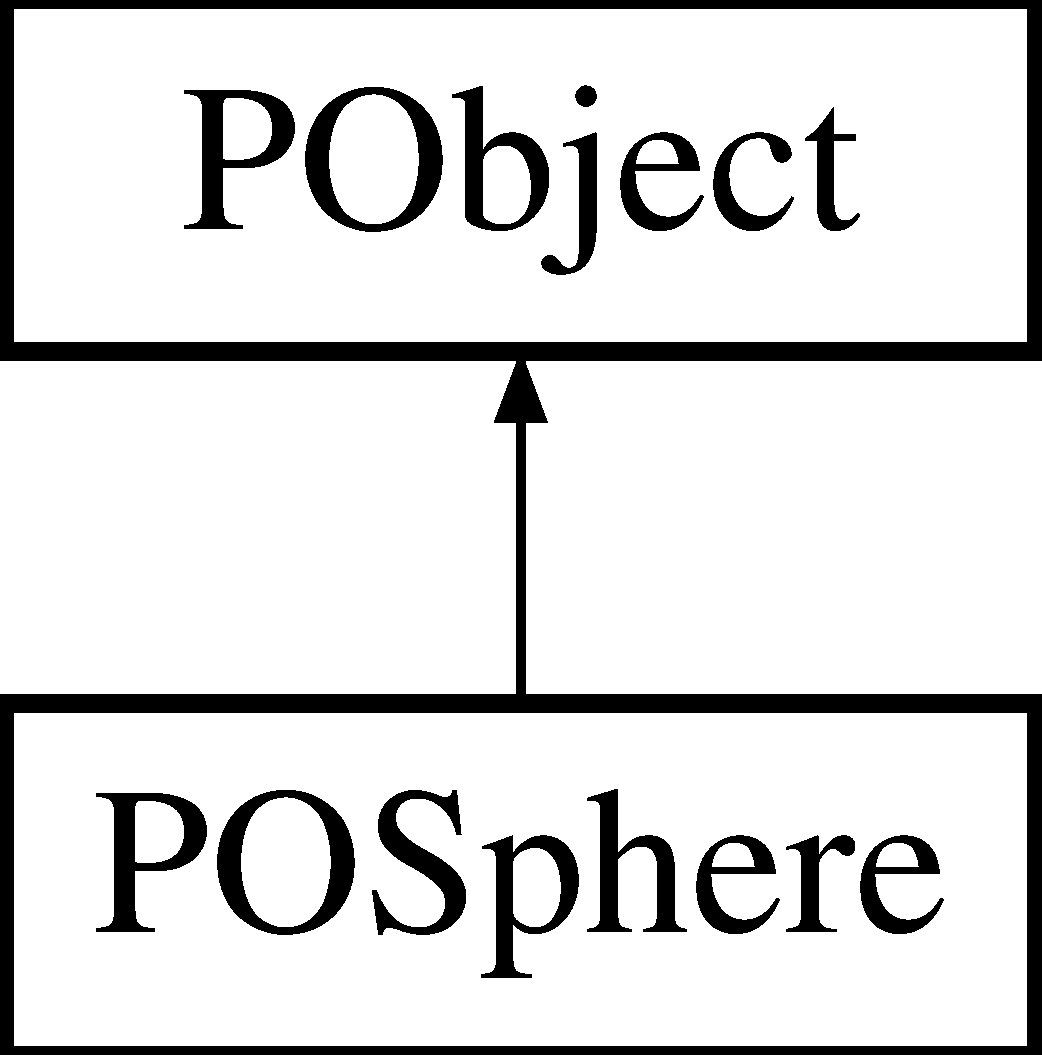
\includegraphics[height=2cm]{classPOSphere}
\end{center}
\end{figure}
\subsection*{Public Member Functions}
\begin{CompactItemize}
\item 
void \hyperlink{classPOSphere_17904f3eeceb2ba07931d6d359bbeebe}{update} ()
\begin{CompactList}\small\item\em default base destructer \item\end{CompactList}\item 
Scalar \hyperlink{classPOSphere_798625bc33390f84032dd30b5abaa112}{detectCollision} (\hyperlink{classPObject}{PObject} $\ast$object)
\begin{CompactList}\small\item\em pure virtual detect collision \item\end{CompactList}\item 
varList \hyperlink{classPOSphere_cab4d5434c63870cd383d38eb985a4fd}{getStats} ()
\begin{CompactList}\small\item\em pure virtual get Statistics for the object \item\end{CompactList}\item 
\hypertarget{classPOSphere_39a1a0d77b89ead931e6bef08d41bdd0}{
void \hyperlink{classPOSphere_39a1a0d77b89ead931e6bef08d41bdd0}{setStats} (varList \_\-stats)}
\label{classPOSphere_39a1a0d77b89ead931e6bef08d41bdd0}

\begin{CompactList}\small\item\em pure virtual set stats \item\end{CompactList}\end{CompactItemize}
\subsection*{Protected Attributes}
\begin{CompactItemize}
\item 
\hypertarget{classPOSphere_d9ae7837bb073b0e88c2def2b3b69412}{
Scalar \textbf{radius}}
\label{classPOSphere_d9ae7837bb073b0e88c2def2b3b69412}

\end{CompactItemize}


\subsection{Detailed Description}
Class for sphere Physics Objects. 

This is the math base for the mathematic simplistic representation of spherical physics based objects 

\subsection{Member Function Documentation}
\hypertarget{classPOSphere_17904f3eeceb2ba07931d6d359bbeebe}{
\index{POSphere@{POSphere}!update@{update}}
\index{update@{update}!POSphere@{POSphere}}
\subsubsection[update]{\setlength{\rightskip}{0pt plus 5cm}void POSphere::update ()\hspace{0.3cm}{\tt  \mbox{[}virtual\mbox{]}}}}
\label{classPOSphere_17904f3eeceb2ba07931d6d359bbeebe}


default base destructer 

pure virtual update 

Implements \hyperlink{classPObject_587e0263ce46133bf886729f890f9f2b}{PObject}.\hypertarget{classPOSphere_798625bc33390f84032dd30b5abaa112}{
\index{POSphere@{POSphere}!detectCollision@{detectCollision}}
\index{detectCollision@{detectCollision}!POSphere@{POSphere}}
\subsubsection[detectCollision]{\setlength{\rightskip}{0pt plus 5cm}Scalar POSphere::detectCollision ({\bf PObject} $\ast$ {\em object})\hspace{0.3cm}{\tt  \mbox{[}virtual\mbox{]}}}}
\label{classPOSphere_798625bc33390f84032dd30b5abaa112}


pure virtual detect collision 

This is the function that we will use to figure out the distance from another object and thus if we collided with it \begin{Desc}
\item[Returns:]Scalar value that is $>$0 if there is no collision =0 if they are just touching and $<$0 if they have hit to intersection(hit with force) \end{Desc}
\begin{Desc}
\item[Parameters:]
\begin{description}
\item[{\em brings}]in a pointer to a physics object to test for distance/collision \end{description}
\end{Desc}


Implements \hyperlink{classPObject_e1828c1830e8e9924ca4c560cbe2f933}{PObject}.\hypertarget{classPOSphere_cab4d5434c63870cd383d38eb985a4fd}{
\index{POSphere@{POSphere}!getStats@{getStats}}
\index{getStats@{getStats}!POSphere@{POSphere}}
\subsubsection[getStats]{\setlength{\rightskip}{0pt plus 5cm}varList POSphere::getStats ()\hspace{0.3cm}{\tt  \mbox{[}virtual\mbox{]}}}}
\label{classPOSphere_cab4d5434c63870cd383d38eb985a4fd}


pure virtual get Statistics for the object 

This is the function that we will use to get the object's data for the objects \begin{Desc}
\item[Returns:]returns a list of stats. The first is the type ID. \end{Desc}
\begin{Desc}
\item[Parameters:]
\begin{description}
\item[{\em none}]\end{description}
\end{Desc}


Implements \hyperlink{classPObject_4def469478987ead107c777d31790092}{PObject}.

The documentation for this class was generated from the following file:\begin{CompactItemize}
\item 
pobject.h\end{CompactItemize}

\printindex
\end{document}
